\begin{figure}[h]
    \begin{center}
    \vspace{-1em}
    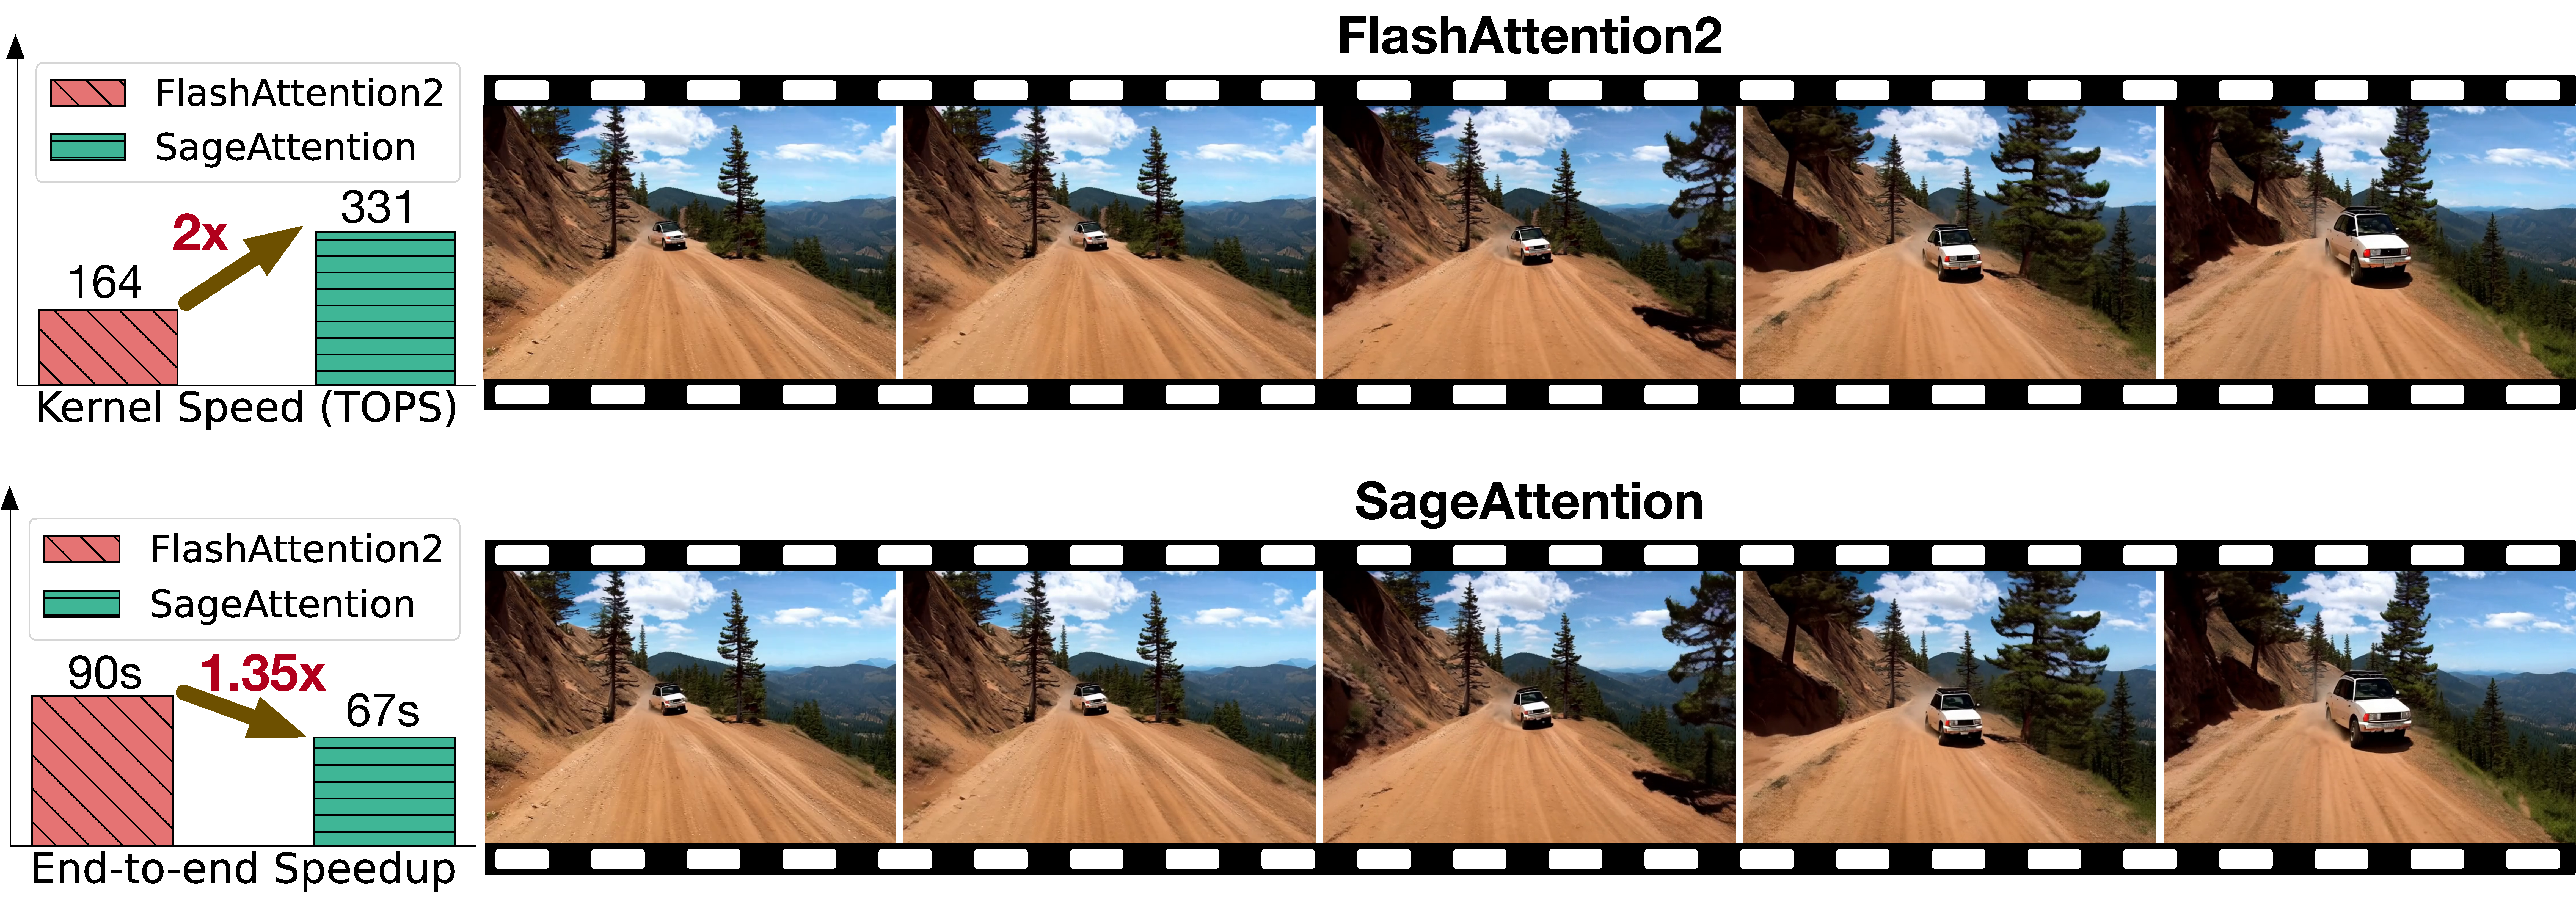
\includegraphics[width=0.99\textwidth]{figs/Intro.pdf}
    \vspace{-.6em}
    \caption{An example of \our on video generation (CogvideoX on RTX4090).}
    \vspace{-.6em}
    \end{center}
    \label{fig:intro}
\end{figure}



\section{Introduction}

Attention is the fundamental component of transformers~\citep{vaswani2017attention}, and efficiently computing attention is crucial for transformer-based applications. 
Moreover, there is a recent trend in processing longer sequences, which further strengthens the need for faster attention. In tasks like video generation~\citep{yang2024cogvideox} and language model prefilling~\citep{llama31model}, the sequence length can easily go up to 8K$\sim$ 128K. Due to its quadratic complexity, the cost of attention dominates all other operations in such scenarios, as illustrated in Figure~\ref{fig:motivation}. 


\begin{figure}[h]
    \centering 
    \begin{minipage}[b]{0.42\linewidth} 
        \centering
        \vspace{-.2em}
        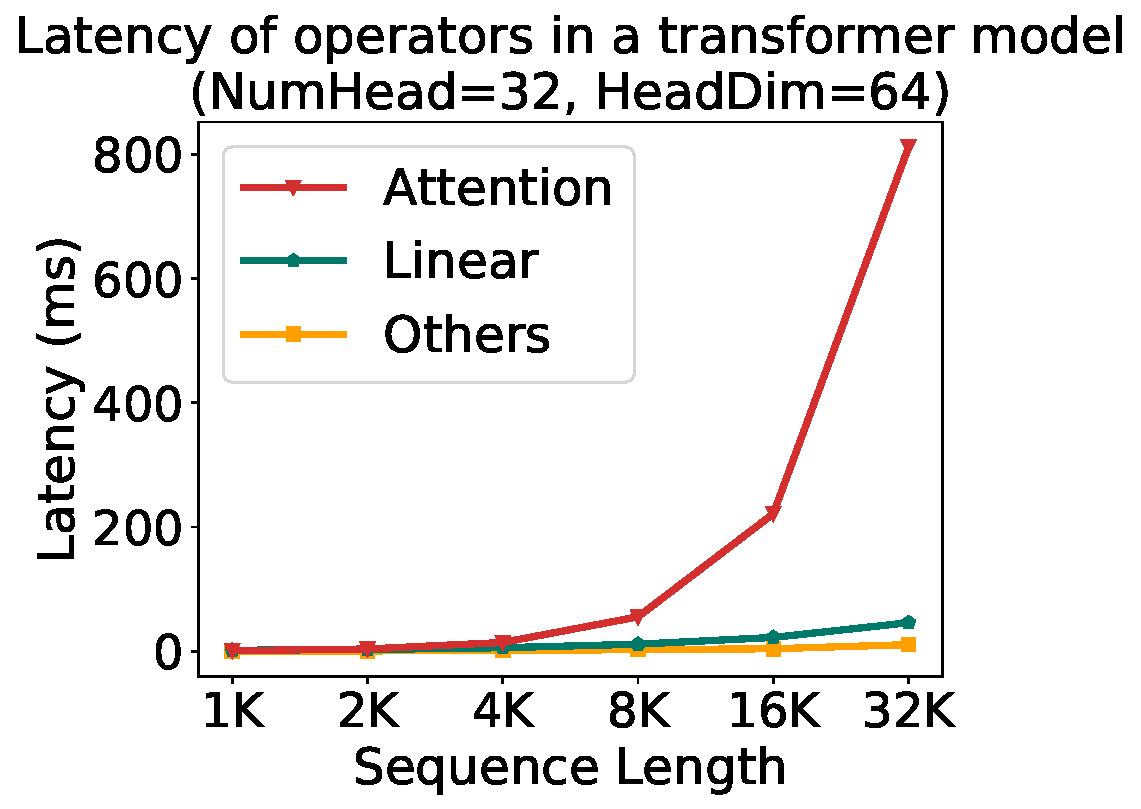
\includegraphics[width=0.93\linewidth]{figs/motivation.pdf} 
        \vspace{-.7em}
        \caption{Latency of attention.}
        \label{fig:motivation}
    \end{minipage}
    \hspace{0.05\textwidth} 
    \begin{minipage}[b]{0.37\linewidth}
        \centering
        \vspace{-.2em}
        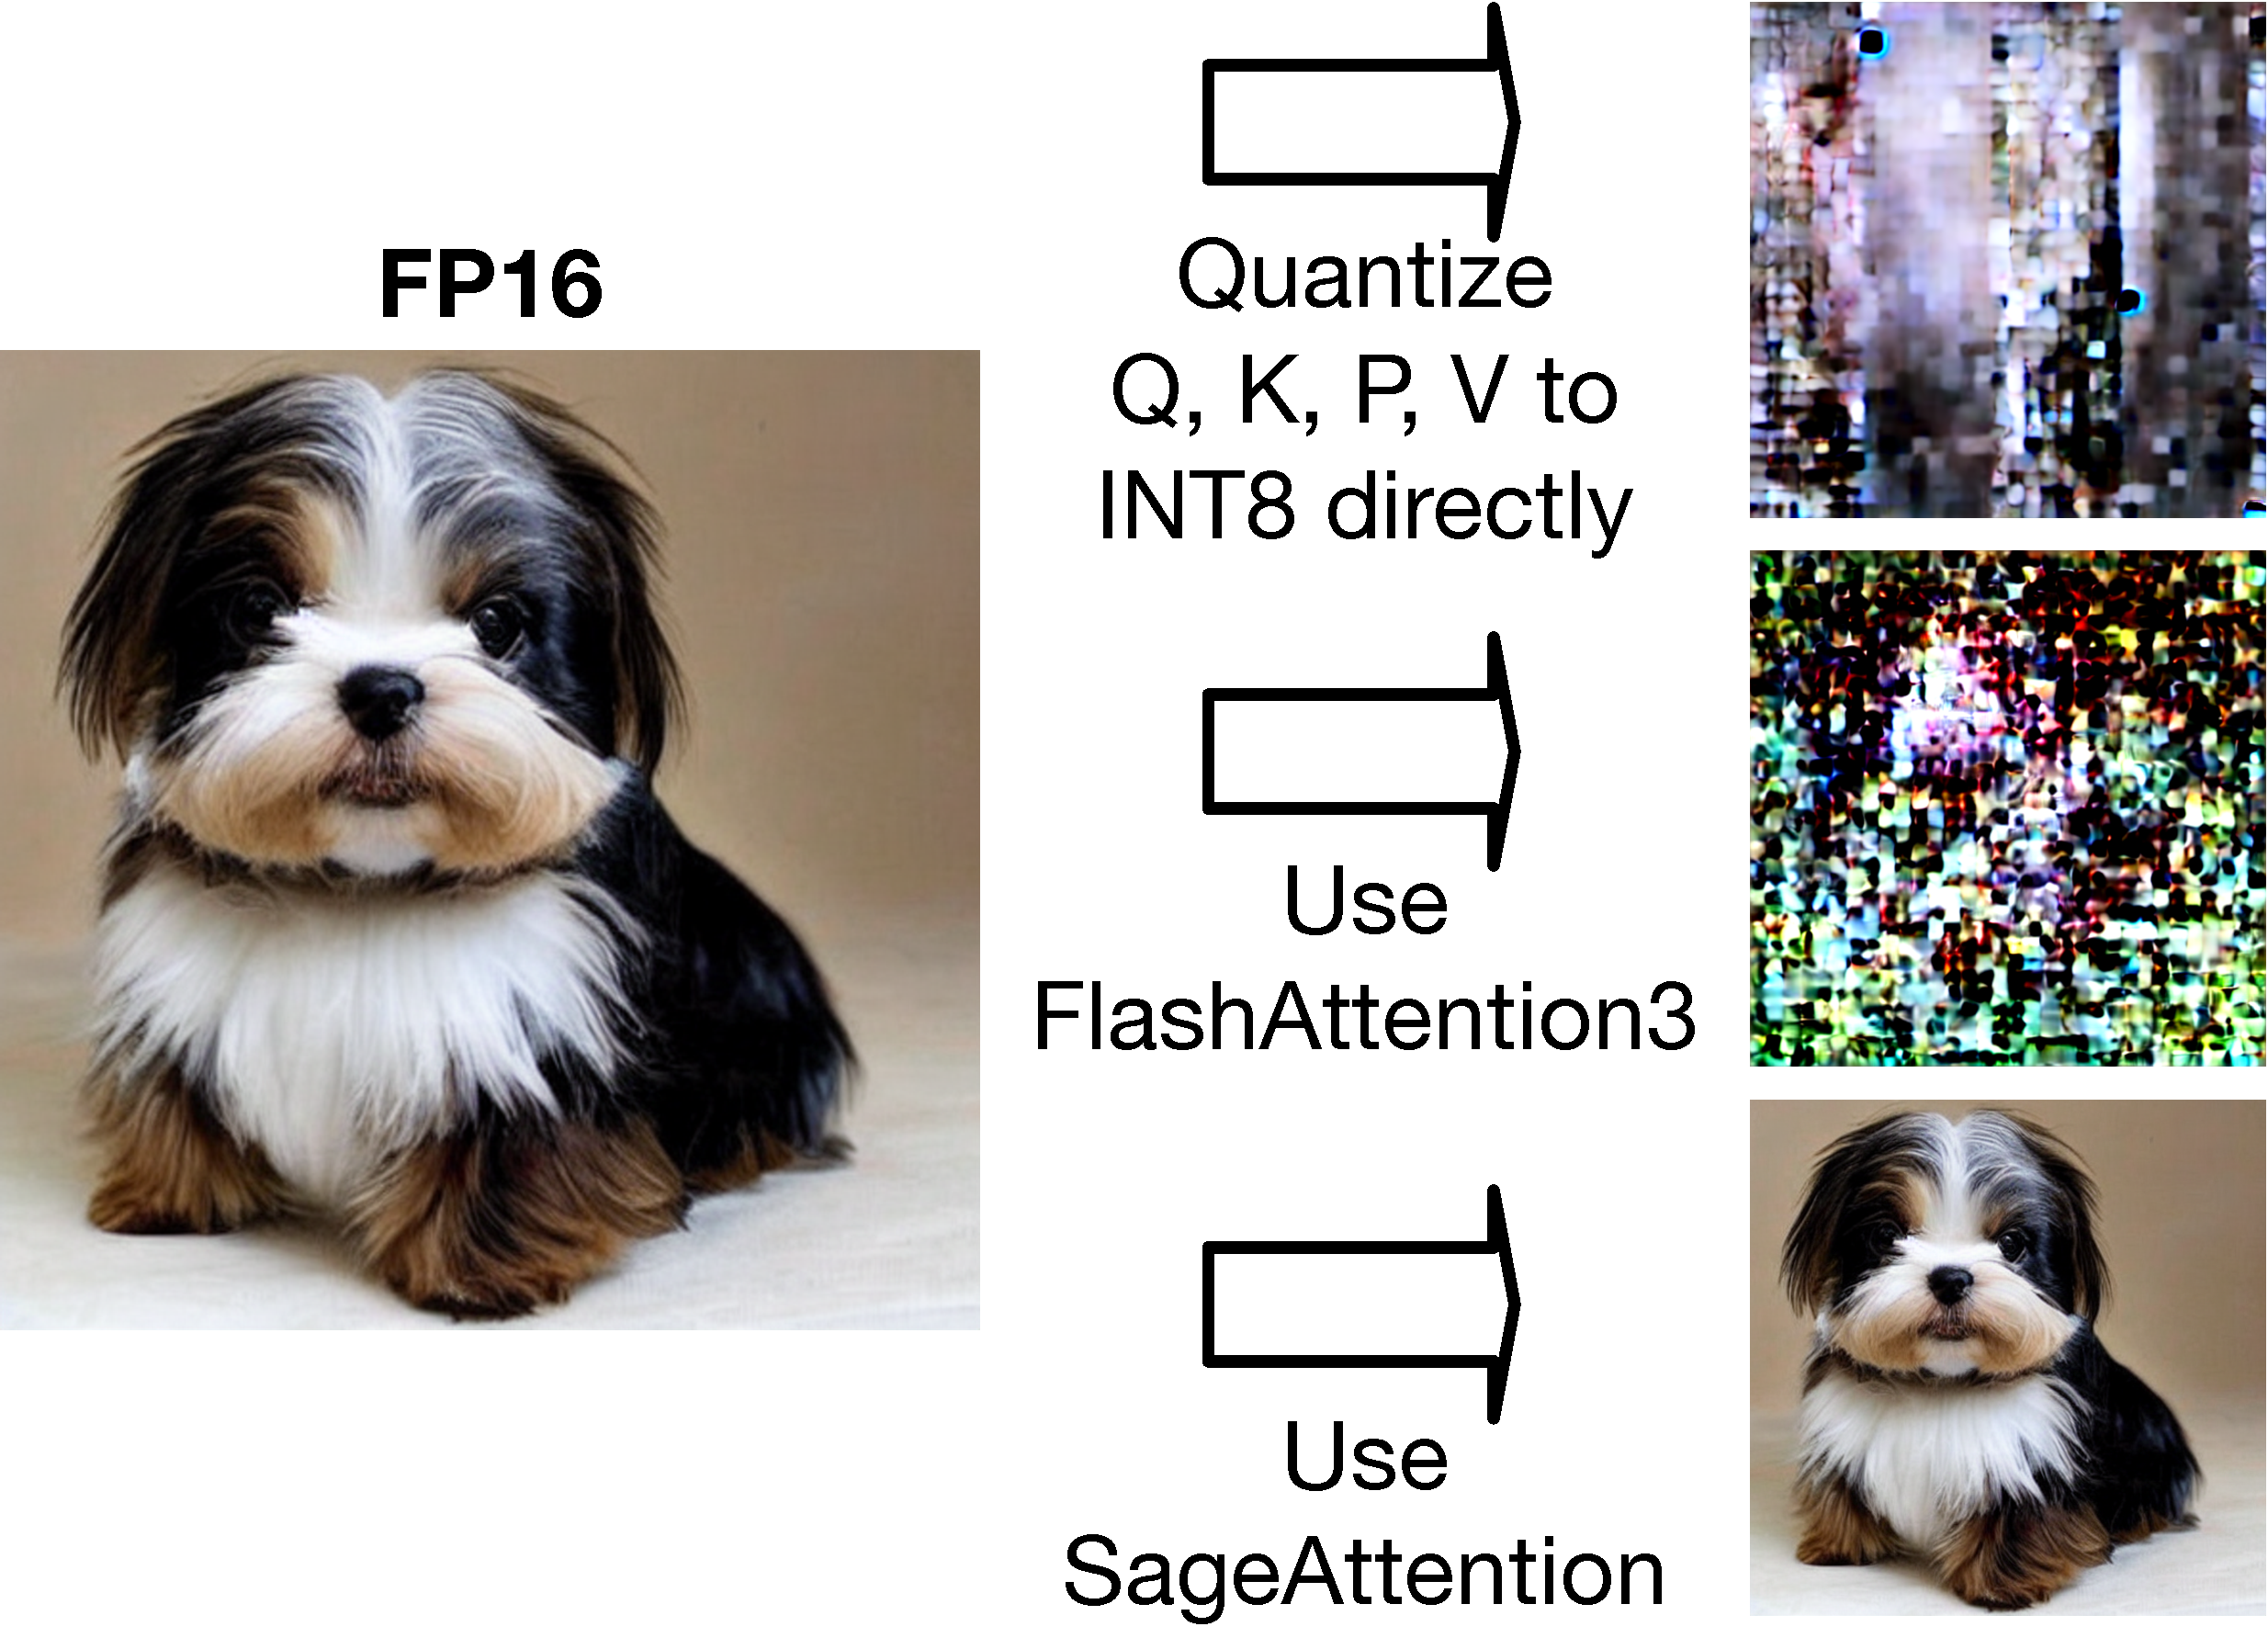
\includegraphics[width=\linewidth]{figs/challenge.pdf} 
        \vspace{-1.7em}
        \caption{A comparison example.}
        \label{fig:challenge}
    \end{minipage}
\vspace{-1.3em}
\end{figure}


Quantization is an effective strategy for enhancing neural networks' computational and memory efficiency by reducing the numerical precision. There are abundant works on accelerating training~\citep{sun2019hybrid,xijetfire,peng2023fp8} and inference~\citep{jacob2018quantization,xiao2023smoothquant} with low-precision numerical formats such as FP8, INT8, or INT4. However, existing works primarily focused on quantizing the \emph{linear} layer, where \emph{attention} is left unaccelerated in high-precision, such as FP16. There is not yet a work that systematically investigates the quantization of attention. 
Moreover, many quantization methods require extra training, and the cost can be prohibitive for large-scale models. 
While \purple{FlashAttention3}~\citep{shah2024flashattention} was released recently and offers an FP8 version, it is \purple{tailored to and can only be used with the Nvidia Hopper architecture}. This exclusive optimization limits its broader applicability. Furthermore, our analysis demonstrates that directly implementing the FP8 version can lead to performance degradation, as detailed in Table~\ref{tab:quant_type_analysis}.



Quantizing attention is challenging. The computation of attention is more complex than that of linear operations. Attention includes a softmax operation and two matrix multiplication (Matmul) operations: $QK^\top$ and $PV$. Direct 8-bit quantization and dequantization of the matrices $(Q, K, P, V)$ in attention will result in significantly degraded performance across various models. For example, the text-to-image model Unidiffuser~\citep{bao2022uni} will generate a completely blurry image with both INT8 and FlashAttention3's FP8 implementation (See Figure~\ref{fig:challenge}), and Llama2 only achieves a random-guessing-level accuracy of 25.5\% on the MMLU dataset with INT8 attention. After investigating deeply, we identified two primary challenges: 
\textbf{(C1)} The matrix $K$ exhibits a significant channel-wise outlier, leading to substantial accuracy loss during quantization.
\textbf{(C2)} Simply quantizing $(P, V)$ into INT8 does not consistently ensure the accuracy of $PV$ across various scenarios.

In this paper, we propose \our, a quantization method to accelerate attention while \emph{preserving accuracy}. \our is easy-to-use. As a post-training quantization method, it can be \emph{used in a plug-and-play manner in inference time} by simply replacing the original high-precision implementation. We propose several techniques to achieve this goal. 
First, we opt to quantize the tensors in attention to INT8 rather than FP8. This decision is based on the fact that INT8 Matmul on some commonly used GPUs, e.g., RTX4090 and 3090, are four times faster than in FP16 and two times faster than FP8. Moreover, INT8 quantization for matrices $(Q, K)$ is more precise than FP8 in attention (See Table~\ref{tab:quant_precision_analysis1}).
To address \textbf{(C1)}, we propose a method to smooth the $K$ matrix. This method significantly enhances accuracy with a negligible time overhead ($<$0.2\%). 
To address \textbf{(C2)}, as an alternative to quantizing $(P, V)$ to 8-bit, we propose a more accurate yet efficient method for the Matmul $PV$: we maintain $(P, V)$ in FP16 and use a low-precision FP16 accumulator. This strategy doubles Matmul's speed without sacrificing any accuracy.
Finally, we implement several versions of attention with different speed-accuracy tradeoffs and propose a method to select the fastest attention implementation for each layer while preserving accuracy. 

We offer a high-performance implementation of \our on RTX4090 and 3090 GPUs using Triton~\citep{openaitriton}. Our implementation contains a fused kernel combining ROPE with quantization and a fast self-attention kernel inspired by FlashAttention-style tiling. The implementation utilizes the fast INT8 \emph{mma(u8.u8.s32)} and FP16-with-FP16-accumulator \emph{mma(f16.f16.f16)} instructions of Nvidia Tensor Core.
Our kernel is about $2.1 \times$ and $2.7 \times$ faster than FlashAttention2 and xformers, respectively.
Notably, it achieves 340 TOPS on RTX4090 at headdim=64 and headdim=128, reaching 52\% of the theoretical INT8 throughput. In contrast, the peak for the state-of-the-art FlashAttention2 is only 165 TOPS. Moreover, at headdim=64, our throughput on RTX 4090 is even close to the 490 TOPS throughput of FlashAttention3, which is exclusive to the much more powerful and expensive Hopper GPUs.
We extensively evaluate the end-to-end metrics of our approach on state-of-the-art image/video generation, image classification, and language models. On all tasks, \our can be directly adopted in a plug-and-play manner with negligible loss in model performance, while offering more than 2$\times$ speedup than FlashAttention2 and xformers.

